\documentclass[10pt]{article}
\usepackage{upgreek}
\usepackage{amsmath}
\usepackage{graphicx}
\usepackage{subfig}
\usepackage{hyperref}
\usepackage{mathrsfs}
\usepackage{amssymb}
\usepackage{caption}
\usepackage{tikz}
\usepackage{verbatim}
\usetikzlibrary{shapes.geometric, arrows}

\tikzstyle{startstop} = [rectangle, rounded corners, minimum width=3cm, minimum height=1cm,text centered, draw=black, fill=red!30]
\tikzstyle{io} = [trapezium, trapezium left angle=70, trapezium right angle=110, minimum width=3cm, minimum height=1cm, text centered, draw=black, fill=blue!30]
\tikzstyle{process} = [rectangle, minimum width=3cm, minimum height=1cm, text centered, draw=black, fill=orange!30]
\tikzstyle{decision} = [diamond, minimum width=3cm, minimum height=1cm, text centered, draw=black, fill=green!30]
\tikzstyle{arrow} = [thick,->,>=stealth]

\DeclareGraphicsExtensions{.pdf,.png,.jpg,.tif}

\title{Reinforced Fiber Segmenation \\ Blob Detection }

\author{Sungmin Hong}
\date{\today}

\begin{document}
\maketitle

\section*{Summary of the Previous Report}
\label{prev}


The blob detection method using the ratio of Eigenvalues of Hessian matrix was experimented in the previous report(7\_OCT). 
The method depends solely on 2nd derivative of image apporximated by the LoG filter. 
Thus, the method is sensitive to $\sigma$ of LoG filter for detecting blobs and vessels.
Small $\sigma$ results in many false positives for blob detection, especially in vessels which have similar statistical property as blobs. 
On the contrary, large $\sigma$ misses small air blobs even though it is obvious in the sense of intensity. 
Most of vessel-like structure segmentation method set a single $\sigma$ for an entire image, which is inappropriate for air-voids detection. 
To solve the variation of the size of air-voids, I suggested methods which aid the 2nd derivative segmentation method by intensity-based segmentation, or clustering, methods.
I suggested the method using the maximally stable extremal regions(MSER) feature and K-Means clustering for the blob detection. 


\section*{Assumptions}
\label{assumption}

There are a few assumptions on air-voids that I made to detect air-voids from a concrete CT image. 
I do not know this would be always true for every CT image, but I tried to be careful since it restricts the problem.

\begin{enumerate}
 \item Darker than any other components(blocks and fibers) in CT image
 \item Uniformly distributed intensity, which means standard deviation of intensity in air-voids is small
 \item Blob-like shapes 
\end{enumerate}

\section*{Watershed segmentation and K-Means clustering method}
\label{methods}

\begin{figure}[h!tb]
  \centering
    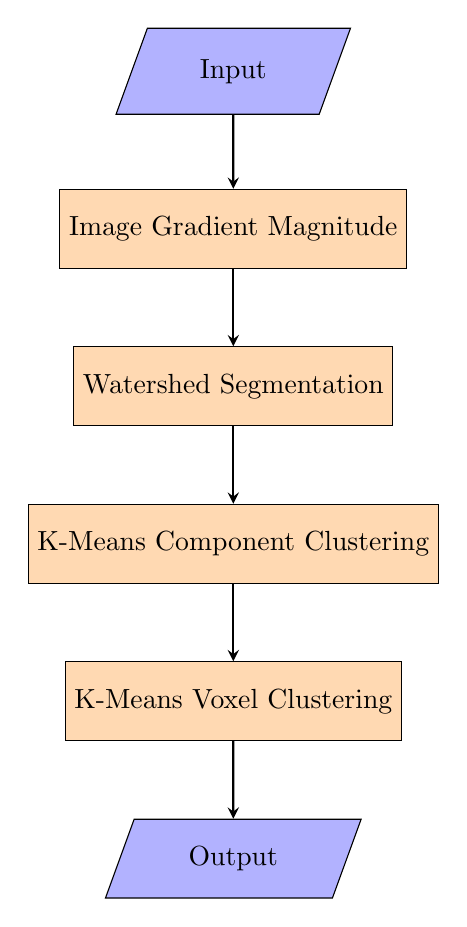
\begin{tikzpicture}[node distance=2cm]
    \node (in1) [io] {Input};
    \node (pro1) [process, below of=in1] {Image Gradient Magnitude};
    \node (pro2) [process, below of=pro1] {Watershed Segmentation};
    \node (pro3) [process, below of=pro2] {K-Means Component Clustering};
    \node (pro4) [process, below of=pro3] {K-Means Voxel Clustering};
    \node (out1) [io, below of=pro4] {Output};

    \draw [arrow] (in1) -- (pro1);
    \draw [arrow] (pro1) -- (pro2);
    \draw [arrow] (pro2) -- (pro3);
    \draw [arrow] (pro3) -- (pro4);
    \draw [arrow] (pro4) -- (out1);
    \label{figFc}
    \end{tikzpicture}
  \caption{Overall work flow of the blob detection algorithm}
\end{figure}

By the first and the second assumptions, I tried the 1st derivative based watershed segmentation for detecting the blob candidates 
and intensity based K-means clustering method for grouping candidates by intensity distribution. Figure~\ref{figFc} describes the over all
flow of the current implemented algorithm.

First, we calculate the graident magnitude of an input image as a valley map for the watershed segmentation algorithm. 
The watershed algorithm with ``proper'' level and threshold generated blobs as shown in Figure~\ref{figGrW}. 

\begin{figure}[h!tb]
  \centering
  \captionsetup[subfigure]{labelformat=empty}
  \subfloat[Input]{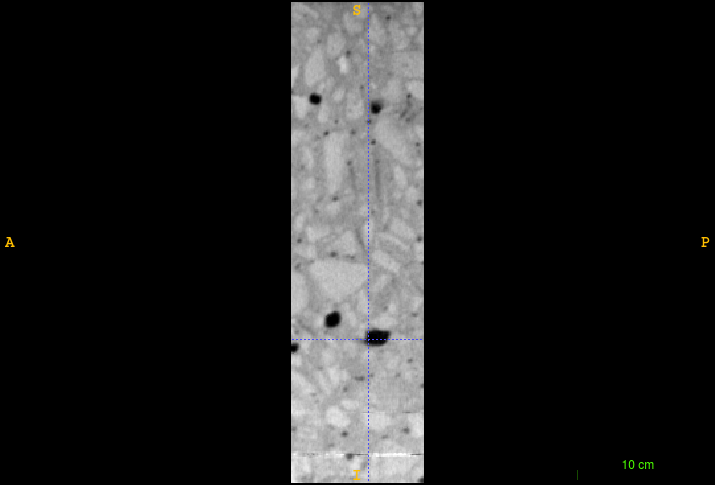
\includegraphics[width=40mm, height=40mm]{Image1.png}}  \hfill
  \subfloat[Gradient Magnitude]{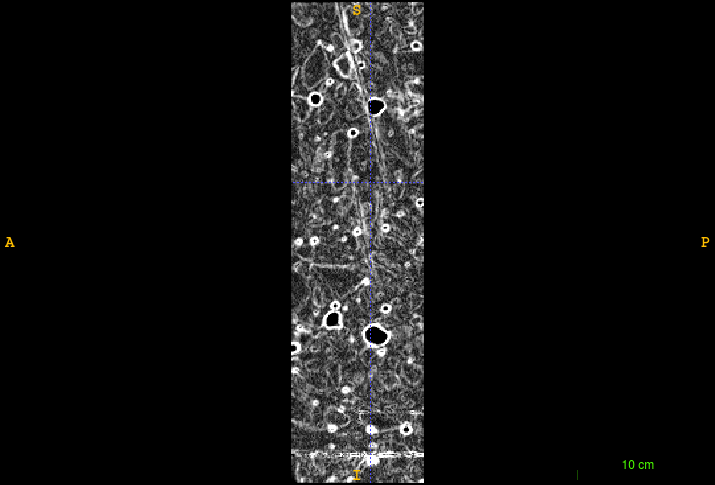
\includegraphics[width=40mm, height=40mm]{Gradient1.png}} \hfill
  \subfloat[Watershed]{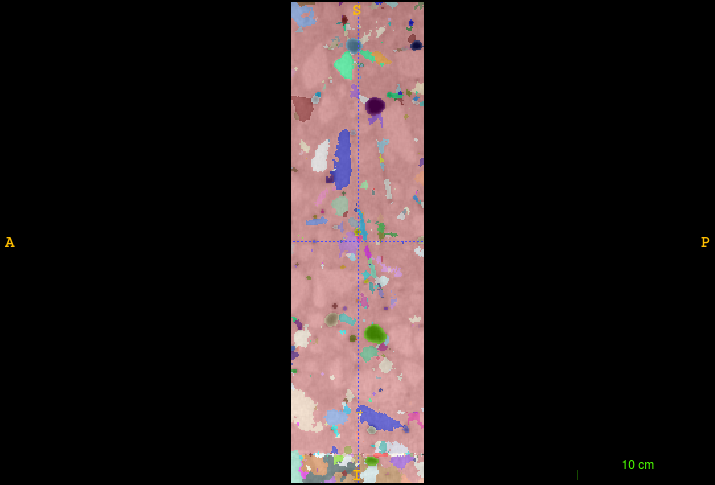
\includegraphics[width=40mm, height=40mm]{Watershed1.png}}  
\caption{Gradient magnitude image and watershed segmentation results}
\label{figGrW}
\end{figure}

I put the result of watershed algorithm into the K-means clustering method with $ K = 4 $, $K$ is decided by the observation to the input image. 
For K-means clustering, the Connected Component Analysis was used to group the adjacent object voxels. 
Then I extracted mean intensity, mean eigenvalues of Hessian matrix (I will discuss about the effect of $\sigma$ of LoG filter in the next section) for 
each component and put them into the clustering methods. As shown in Figure~\ref{figE}, the eigenvalues of each voxel have seperability for blobs.

\begin{figure}[h!tb]
  \centering
  \captionsetup[subfigure]{labelformat=empty}
  \subfloat[Input]{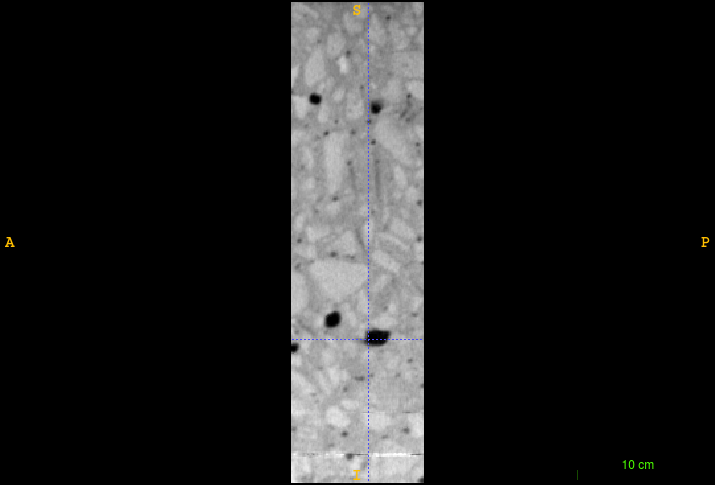
\includegraphics[width=30mm, height=30mm]{Image1.png}}  \hfill
  \subfloat[$\lambda_1$]{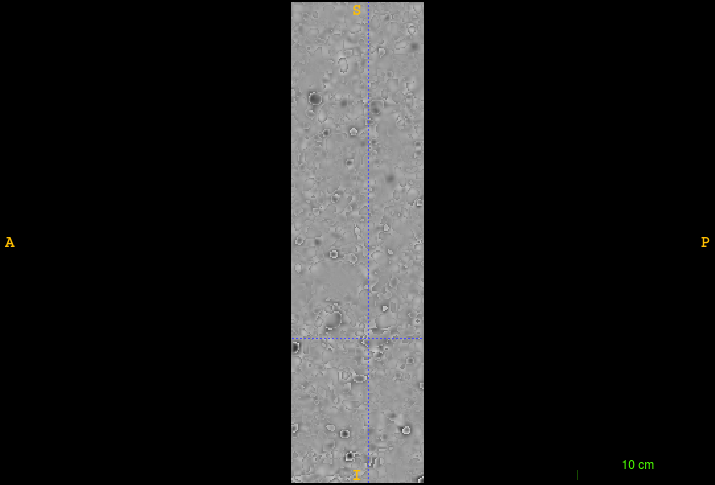
\includegraphics[width=30mm, height=30mm]{E0Sigma21.png}}  \hfill
  \subfloat[$\lambda_2$]{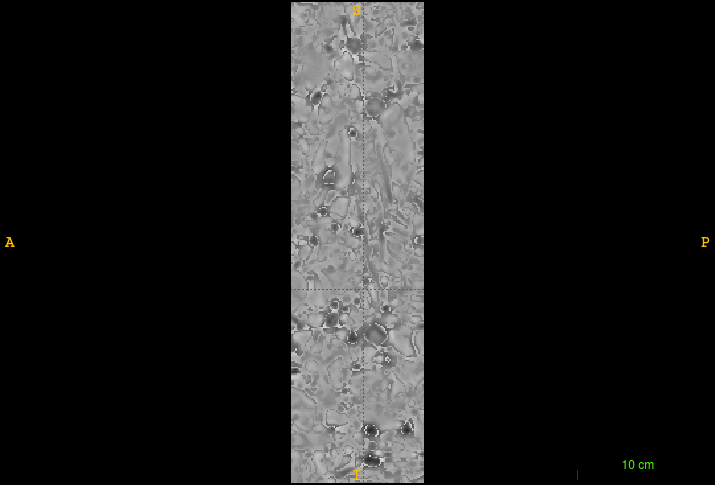
\includegraphics[width=30mm, height=30mm]{E1Sigma21.png}} \hfill
  \subfloat[$\lambda_3$]{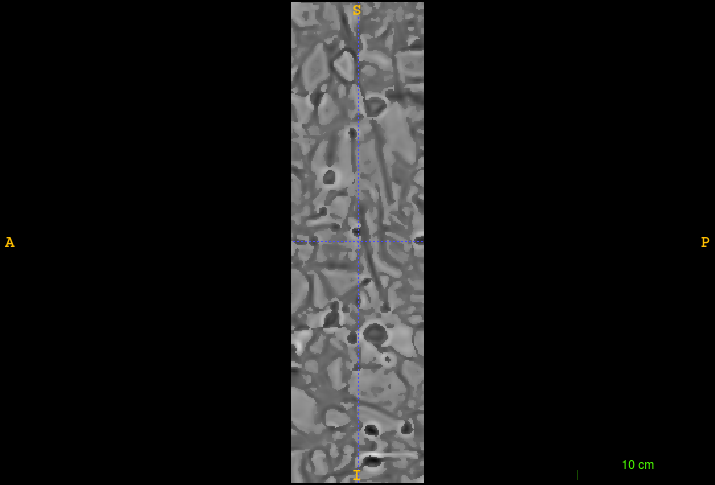
\includegraphics[width=30mm, height=30mm]{E2Sigma21.png}}  
\caption{Input features for 1st K-Means clustering. Intensity and eigenvalue maps of Hessian matrix for each voxel, $\lambda_1 < \lambda_2 < \lambda_3$}
\label{figE}
\end{figure}

\begin{figure}[h!tb]
  \centering
  \captionsetup[subfigure]{}
  \subfloat[Component Clustering]{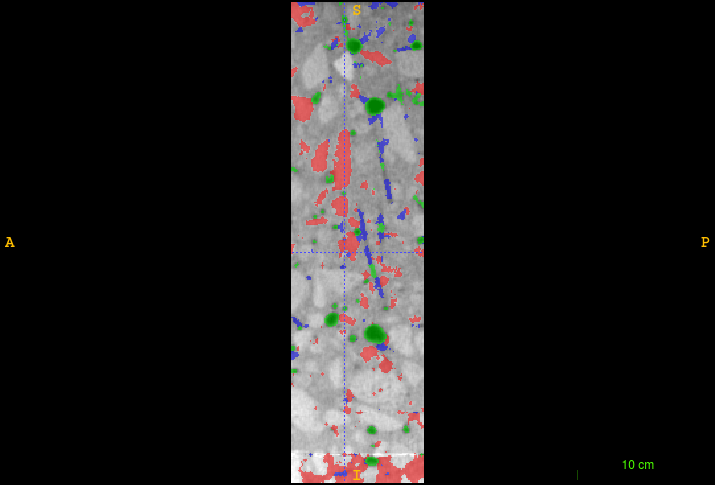
\includegraphics[width=30mm, height=30mm]{1stKMeans1.png}}  \hfill
  \subfloat[Lowest Intensity]{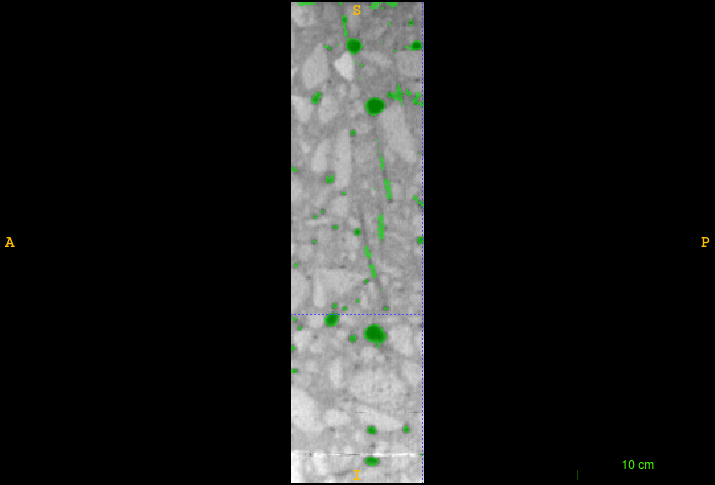
\includegraphics[width=30mm, height=30mm]{1stKMeansLowInten1.png}}  \hfill
  \subfloat[CCA Result]{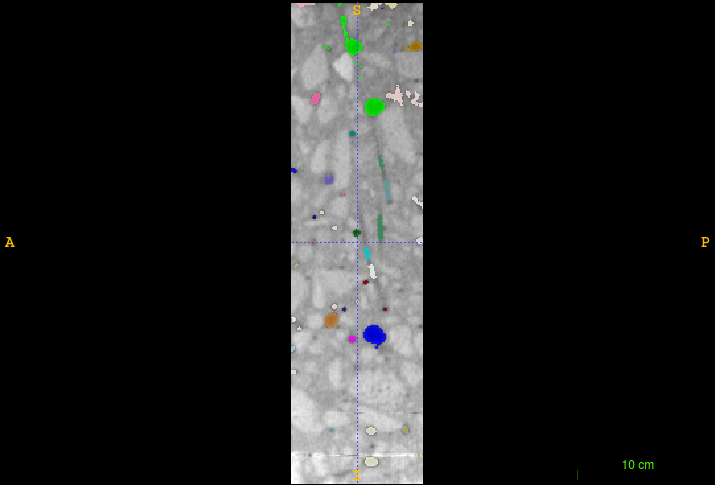
\includegraphics[width=30mm, height=30mm]{1stKMeansLowIntenCCA1.png}} \hfill
  \subfloat[3D CCA]{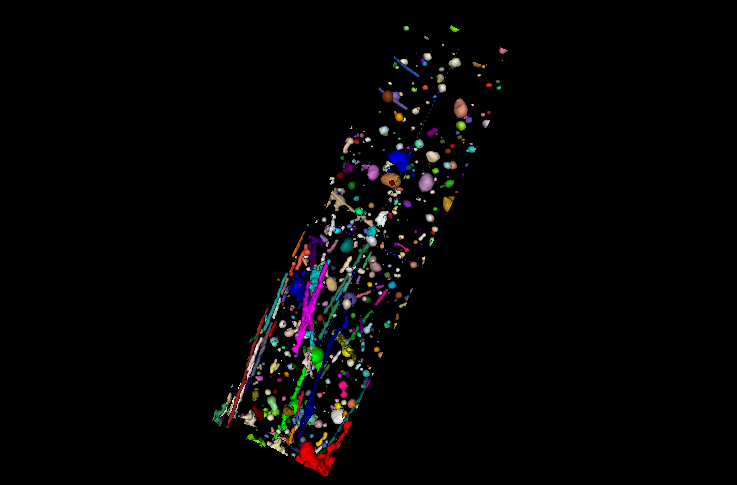
\includegraphics[width=30mm, height=30mm]{1stKMeansLowIntenCCA3D.png}} 
\caption{The result of first K-means clustering}
\label{fig1stK}
\end{figure}

Figure~\ref{fig1stK}(a) shows the result of the first K-means clustering method. Since I assumed that blobs have the lowest intenstity region in the input image,
the cluster with the lowest mean intensity is selected to be processed for the further step. As you can see at Figure~\ref{fig1stK}(c), a single K-means clustering 
captured many false positives in vessel area. It is natural since the first clustering is done to the components which are extracted by watershed segmentation. 
Since the watershed segmentation solely depends on the first derivative, the components do not represent a single object, but a mixture of objects(like blobs, fibers, concretes, and etc.).
Furthremore, if you look at 3D view of the CCA results at Figure~\ref{fig1stK}(d), you can check that vessels at the lower part on z-axis
are more likely to be captured since the intensity is not really uniform on z-axis(Maybe because of long exporsure time on a CT machine).
Thus, I did the second clustering for all voxels of the minimum intensity cluster of the first K-means clustering method. 
I set $K = 2$ for this time, since I only need to distinguish between blobs and vessel fractures in each component. I only used the intensity and the $\lambda_1$ since only those two are supposed to 
be different for vessels and blobs.

\begin{figure}[h!tb]
  \centering
  \captionsetup[subfigure]{}
  \subfloat[Voxel Clustering]{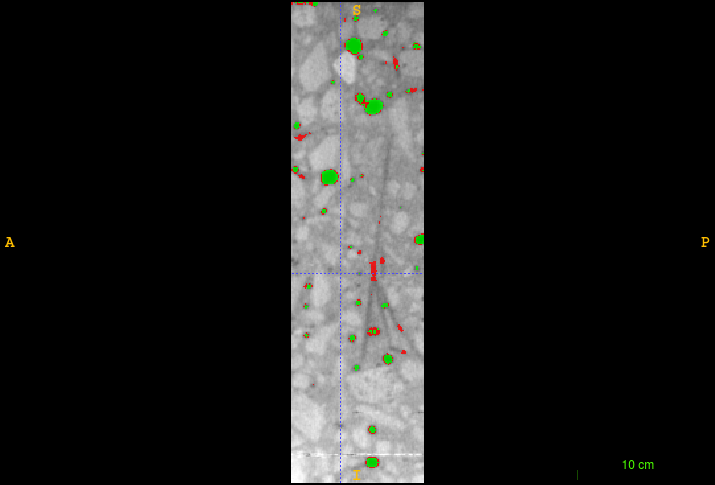
\includegraphics[width=30mm, height=30mm]{2ndKMeans1.png}}  \hfill
  \subfloat[Blob Candidates]{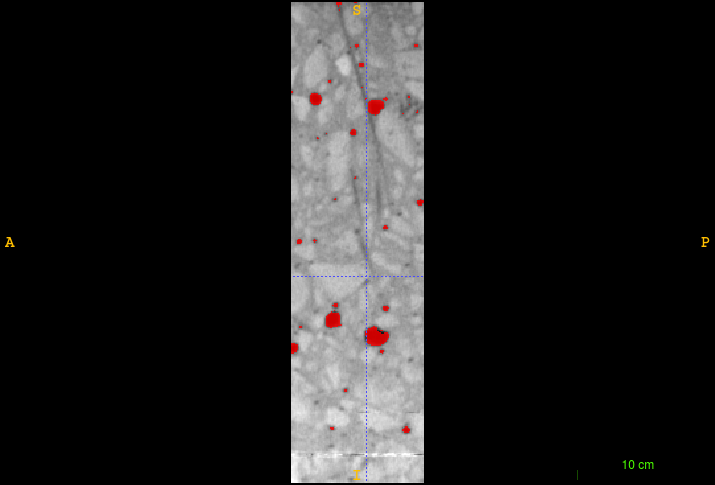
\includegraphics[width=30mm, height=30mm]{2ndKMeansBlob1.png}}  \hfill
  \subfloat[CCA Result]{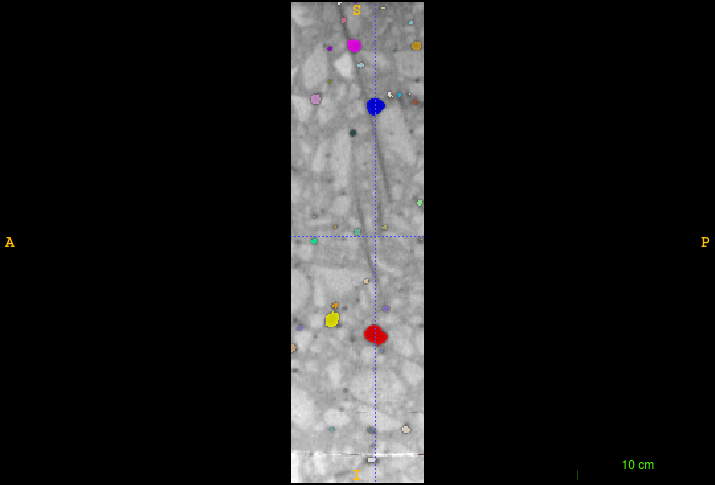
\includegraphics[width=30mm, height=30mm]{2ndKMeansCCA1.png}} \hfill
  \subfloat[3D CCA]{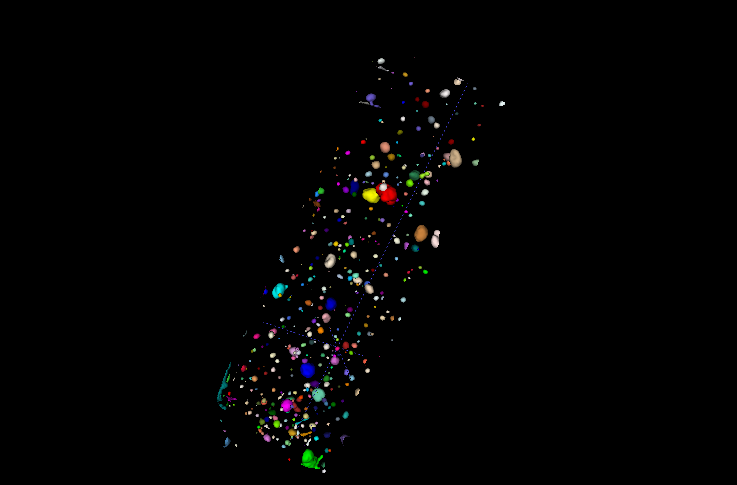
\includegraphics[width=30mm, height=30mm]{2ndKMeansCCA3D.png}} 
\caption{The result of first K-means clustering}
\label{fig2ndK}
\end{figure}

As a result, I could extract blobs for ``StiffFiber\_cropped'' image. The limitations of this method will be discussed in the next section.


\bibliographystyle{unsrt}
\bibliography{FRCBib.bib}

\end{document} 
